\documentclass [11pt, a4wide, twoside]{article}

\usepackage{times}
\usepackage{epsfig}
\usepackage{ifthen}
\usepackage{xspace}
\usepackage{fancyhdr}
\usepackage{hyperref}
\usepackage{pdfpages}
\usepackage{amsmath}
\hypersetup{
    % true means draw the links themselves colored and do not draw a bounding
    % box
    colorlinks=true,
    linkcolor= blue,
    citecolor= blue,
    filecolor=blue,
    urlcolor= blue
}

% solution switch
\newboolean{showsolution}
\setboolean{showsolution}{true} %set it either to true or false


%layout
\topmargin      -5.0mm
\oddsidemargin  6.0mm
\evensidemargin -6.0mm
\textheight 215.5mm
\textwidth      160.0mm
\parindent        1.0em
\headsep          10.3mm
\headheight        12pt
\lineskip    1pt
\normallineskip     1pt

%header
\lhead{Programming Languages \\ 2021}

\rhead{Prof. O. Nierstrasz\\
Mohammadreza Hazhirpasand, Joel Niklaus}
\lfoot{page \thepage}
\rfoot{\today}
\cfoot{}

\renewcommand{\headrulewidth}{0.1pt}
\renewcommand{\footrulewidth}{0.1pt}

\renewcommand{\thesubsection}{\arabic{subsection}}

%enumeration
\newenvironment{myitemize}{%
     \begin{itemize}
     \setlength{\itemsep}{0cm}}
     {\end{itemize}}

\newenvironment{myenumerate}{%
     \begin{enumerate} \setlength{\itemsep}{0cm}}
     {\end{enumerate}}


%solution
\ifthenelse{\boolean{showsolution}}
   {  \newcommand{\solution}[1]{
   	\noindent\underline{\textbf{Answer:}}\\[2mm]
   	 \textsl{#1}
	 \vspace{10pt}
	 \normalsize
	}
  }
  {  \newcommand{\solution}[1]{} }

\newcounter{exnum}
\def\xexercise{\fontsize{12}{10}\fontseries{bx}\selectfont}
\def\xnormal{\fontseries{m}\fontshape{n}\selectfont}


\newcommand{\exercise}[1]{%
     {\addtocounter{exnum}{1}\vskip 0.8cm{\xexercise \noindent Exercise
\arabic{exnum} (#1)} \xnormal} \vskip 0.3cm} 
 \newcommand{\aufgabe}[1]{
     {\addtocounter{exnum}{1}\vskip 0.8cm{\xexercise \noindent Aufgabe
\arabic{exnum} (#1)} \xnormal} \vskip 0.3cm} 

\pagestyle{fancy}


% ===============ABBREVIATIONS==============================
\newcommand{\eg}{\emph{e.g.,}\xspace}
\newcommand{\ie}{\emph{i.e.,}\xspace}
\newcommand{\etc}{\emph{etc.}\xspace}


\begin{document}

% title
\section*{\ifthenelse{\boolean{showsolution}}{Solution}{}\space{} Stack-based Programming}

% - - - - - - - - - - - - - - - - - - - - - - - - - - - - - - - - - - - - - - -

\begin{myitemize}
\item Exercises are given every week on the PL page of the SCG website \\ (\url{http://scg.unibe.ch/teaching/pl})
\item Solutions to each assignment must be sent to \textbf{mohammadreza.hazhirpasand@inf.unibe.ch}
\item The solutions of the assignments are to be delivered before every Thursday at 5 PM. Solutions handed in later than the specified time will not be accepted. In case of serious reasons send an e-mail to  \textbf{mohammadreza.hazhirpasand@inf.unibe.ch}
\end{myitemize}


\subsection*{Exercise 1 (4 points)}

\begin{myitemize}

\item What kinds of stacks does PostScript manage and what are their roles? (1 pts)

\solution{
\begin{enumerate}
\item Operand stack - the most important, since it's used for all computations
\item Dictionary stack - holds sets of local variables to be used by procedures we define
\item Execution stack - hidden from the user; used to manage running procedures
\item Graphics state stack - makes easy for a user to work in different coordinate systems
\end{enumerate}
}

\item What is the way of defining a procedure in the PostScript program? please also define a procedure to calculate the following formula and print the result on the screen : (( x + y ) / 2) * 2
(2 pts)

\solution{Procedures are defined by binding names to executable objects, in a way ``key value def''.}

\textbf{Solution:}
/str 20 string def \\
320 550 moveto \\
/ADDFIVE \{ add 2 div 2 mul \} def \\
9 9 ADDFIVE str cvs show

\item Define a procedure to print 10 random numbers (using loops) and each number must be printed in a new line. \emph{hint: ``rand'' produces random number}  (1 pts)

\small{sample output: \\
684570285 \\
1502883016 \\
252193898 \\
...
}

\textbf{Solution:}
/newLine \{ \\
	currentpoint exch pop \\
	FS 2 add sub \\
	LM exch moveto \\
\} def \\

/loopit \{ \\
320 650 moveto \\
10 \\
\{ \\
rand str cvs show \\
newLine \\
\} repeat \\
\} def \\
loopit




\end{myitemize}

\subsection*{Exercise 2 (2 points)}

Define a procedure in PostScript that will calculate and print the first \texttt{n} \href{https://en.wikipedia.org/wiki/Catalan_number}{Catalan numbers}, where \texttt{n} is an argument on the stack. Catalan numbers are calculated based on the formula $C_{n} = \dfrac{(2n)!}{(n+1)!n!}$.
The call to the procedure should look like \texttt{ n catalan }.
The output should be similar to the one shown in \autoref{fig:catalan} for \texttt{n = 17}.
Please use the provided \href{http://scg.unibe.ch/download/lectures/pl-exercise21/Assignment02-catalan-template.txt}{template} which contains the skeleton of the code, as it will make it easier for you (and us) to check your solution.
Try to define sub-procedures whenever it makes sense. 

\solution{\href{http://scg.unibe.ch/download/lectures/pl-exercise21/Assignment2-catalan-solution.ps}{Catalan numbers - solution.}}

\begin{figure*}[h]
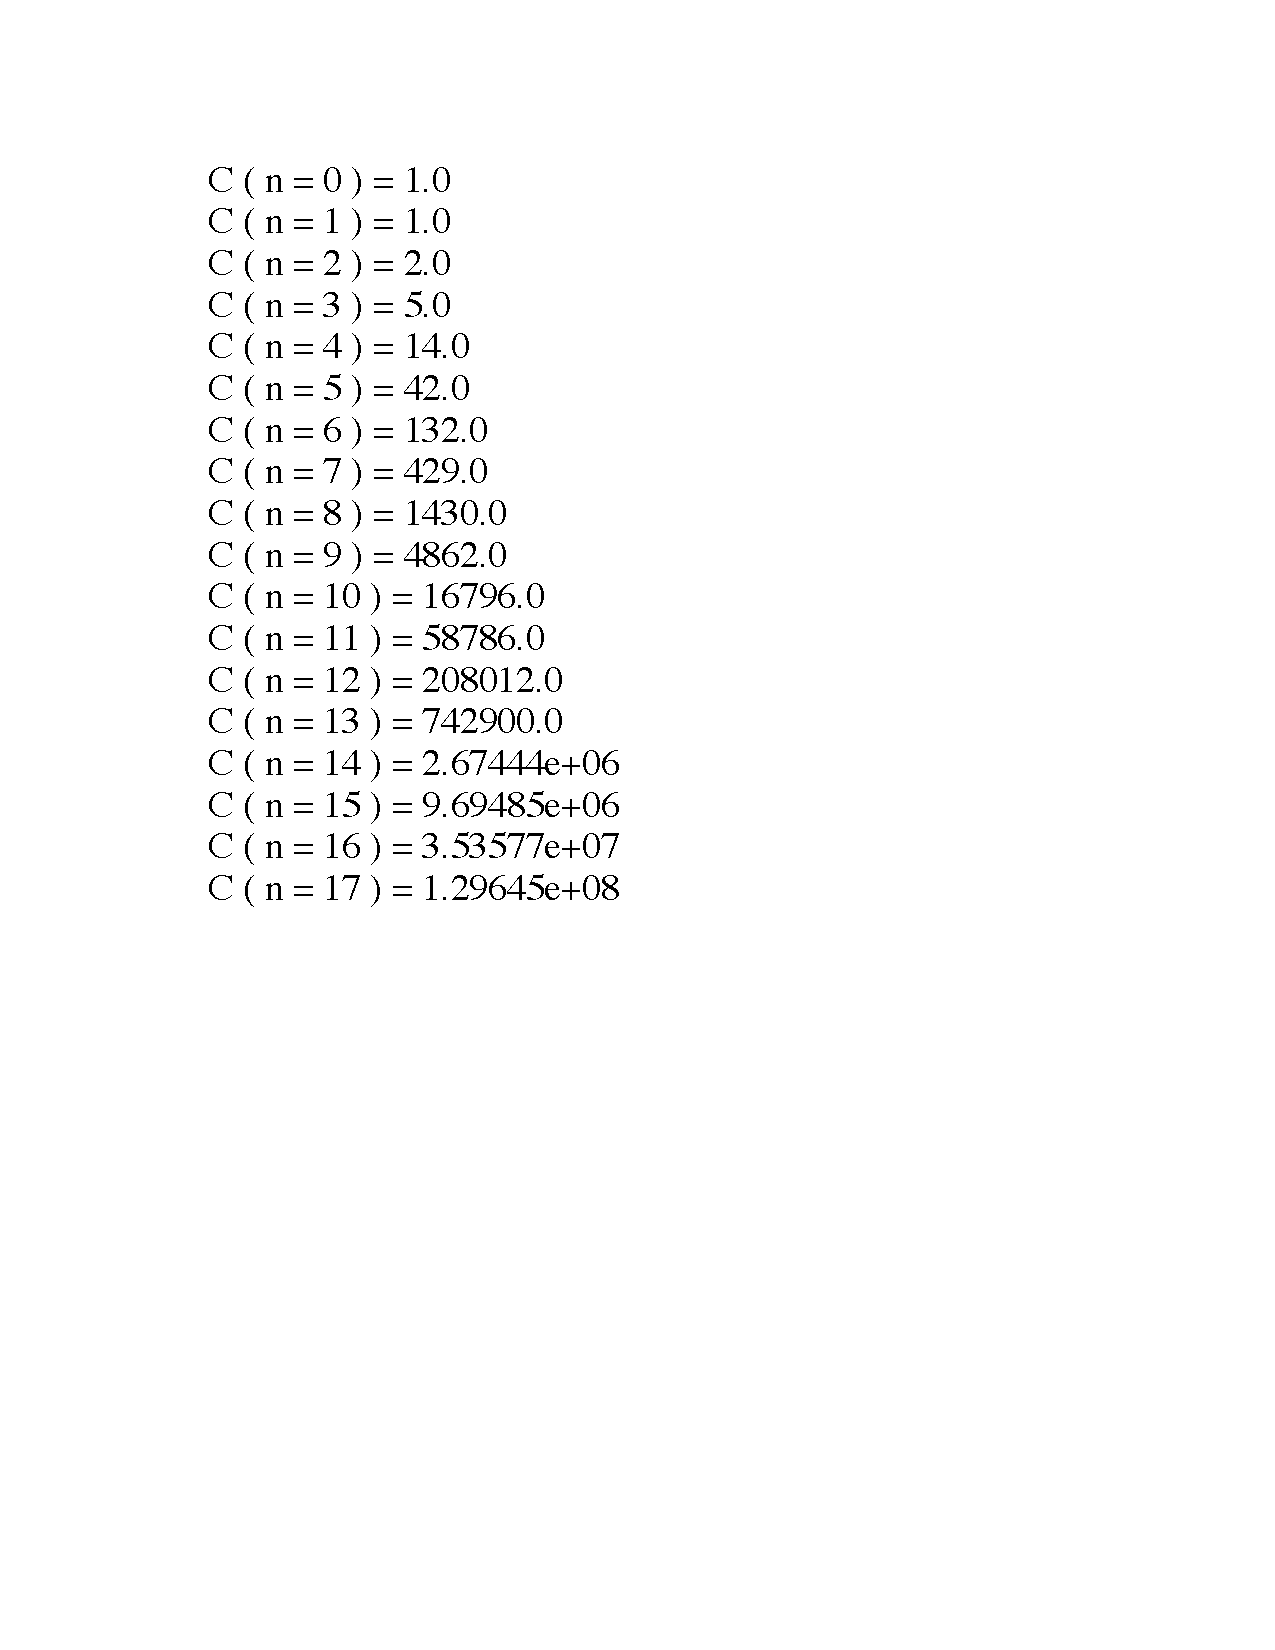
\includegraphics[width=0.358\linewidth]{figs/catalanNumbers.pdf}
\caption{Catalan numbers}
\label{fig:catalan}
\end{figure*}

\end{document}
